% !TEX root = ../agglo_clust_review.tex
% 

\begin{figure}
\centering
        \begin{subfigure}[t]{0.49 \textwidth}
        \centering
        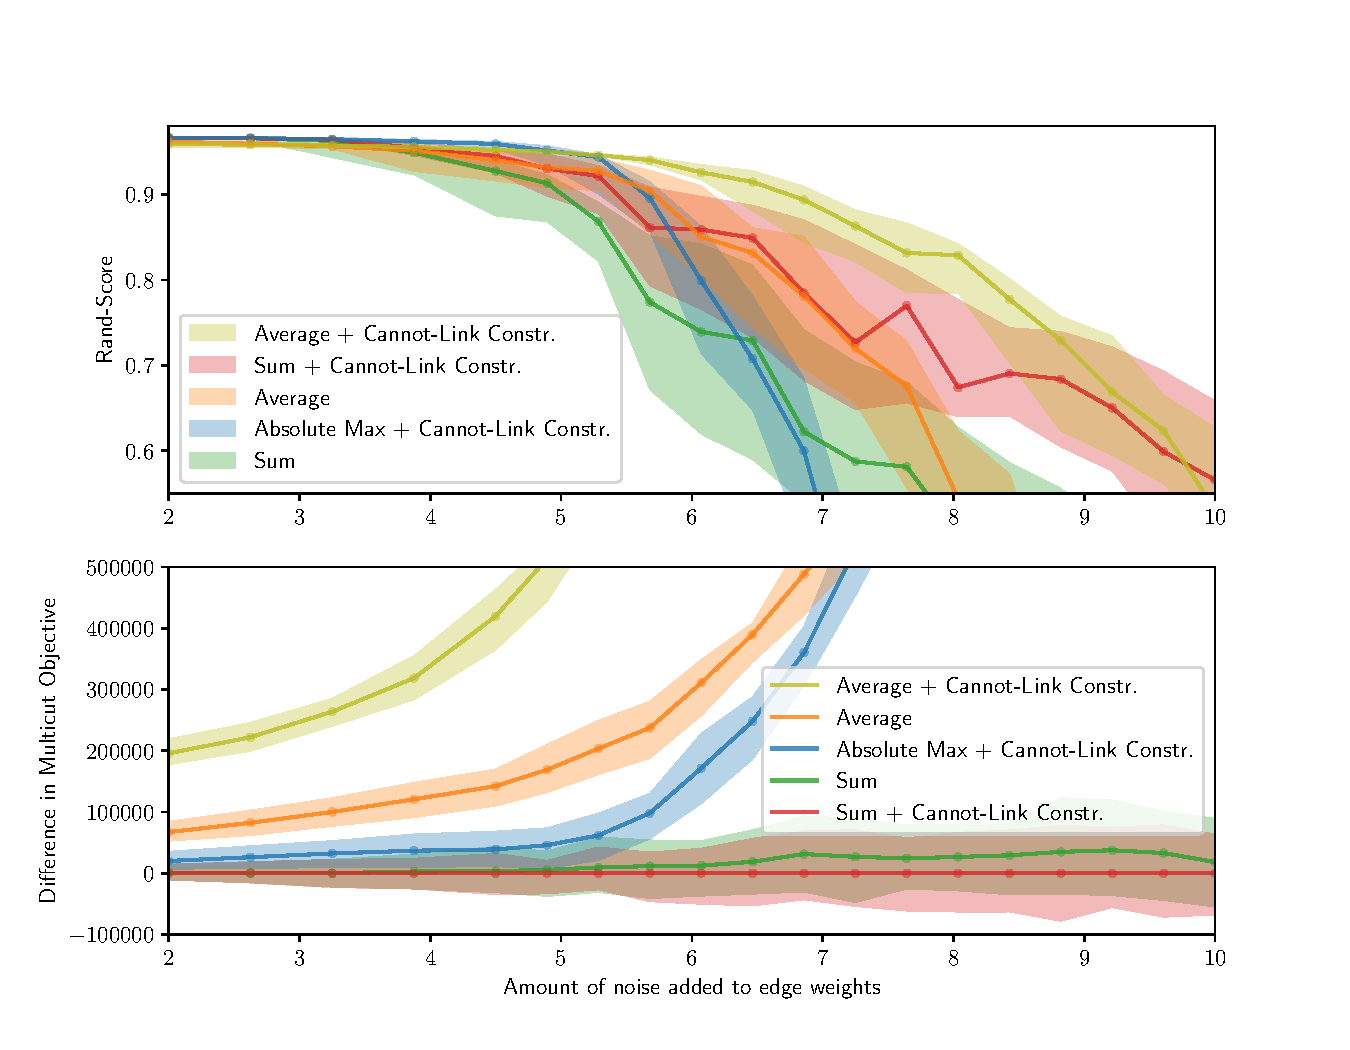
\includegraphics[width=\textwidth,trim=0.55in 0.35in 0.65in 0.80in,clip]{./figs/merge_noise_only_direct.pdf}

        \caption{Without long-range edges: $p_{\mathrm{long}}=0$} \label{fig:merge_noise_only_direct}
    \end{subfigure} \hfill
    \begin{subfigure}[t]{0.49 \textwidth}
        \centering
        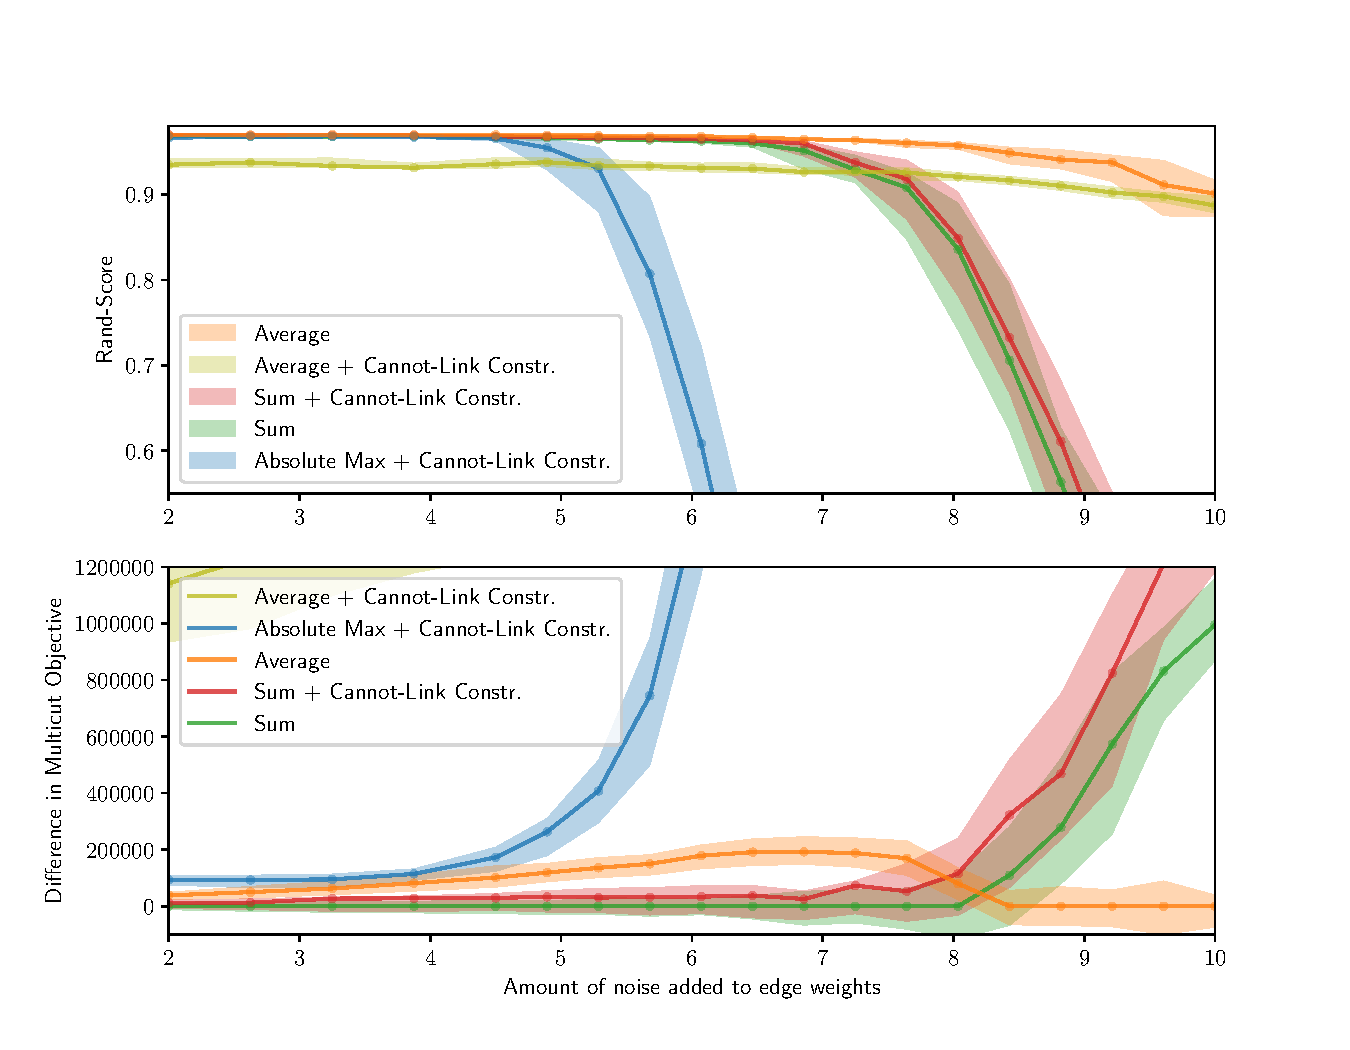
\includegraphics[width=\textwidth,trim=0.53in 0.35in 0.65in 0.80in,clip]{./figs/merge_noise_long_range.pdf}
        \caption{With long-range edges: $p_{\mathrm{long}}=0.1$} \label{fig:merge_noise_with_long_range}
    \end{subfigure}
\caption{Performances of \algname{} with different linkage criteria on a crop of CREMI training data, depending on the amount of noise (x-axis) added to the CNN predictions. \textbf{Top}: Accuracies given by Rand-Score (higher is better). \textbf{Bottom}: Relative difference in multicut objective (lower is better) measuring how balanced the final clusterings are.   
Solid lines represent median values. Values between the 25th and the 75th percentile are shown in shade areas.}\label{fig:noise_plots}
\end{figure}

% \begin{minipage}[b]{0.48\textwidth}
% % \begin{figure}
%         % \begin{subfigure}[t]{0.48 \textwidth}
%         \centering
%         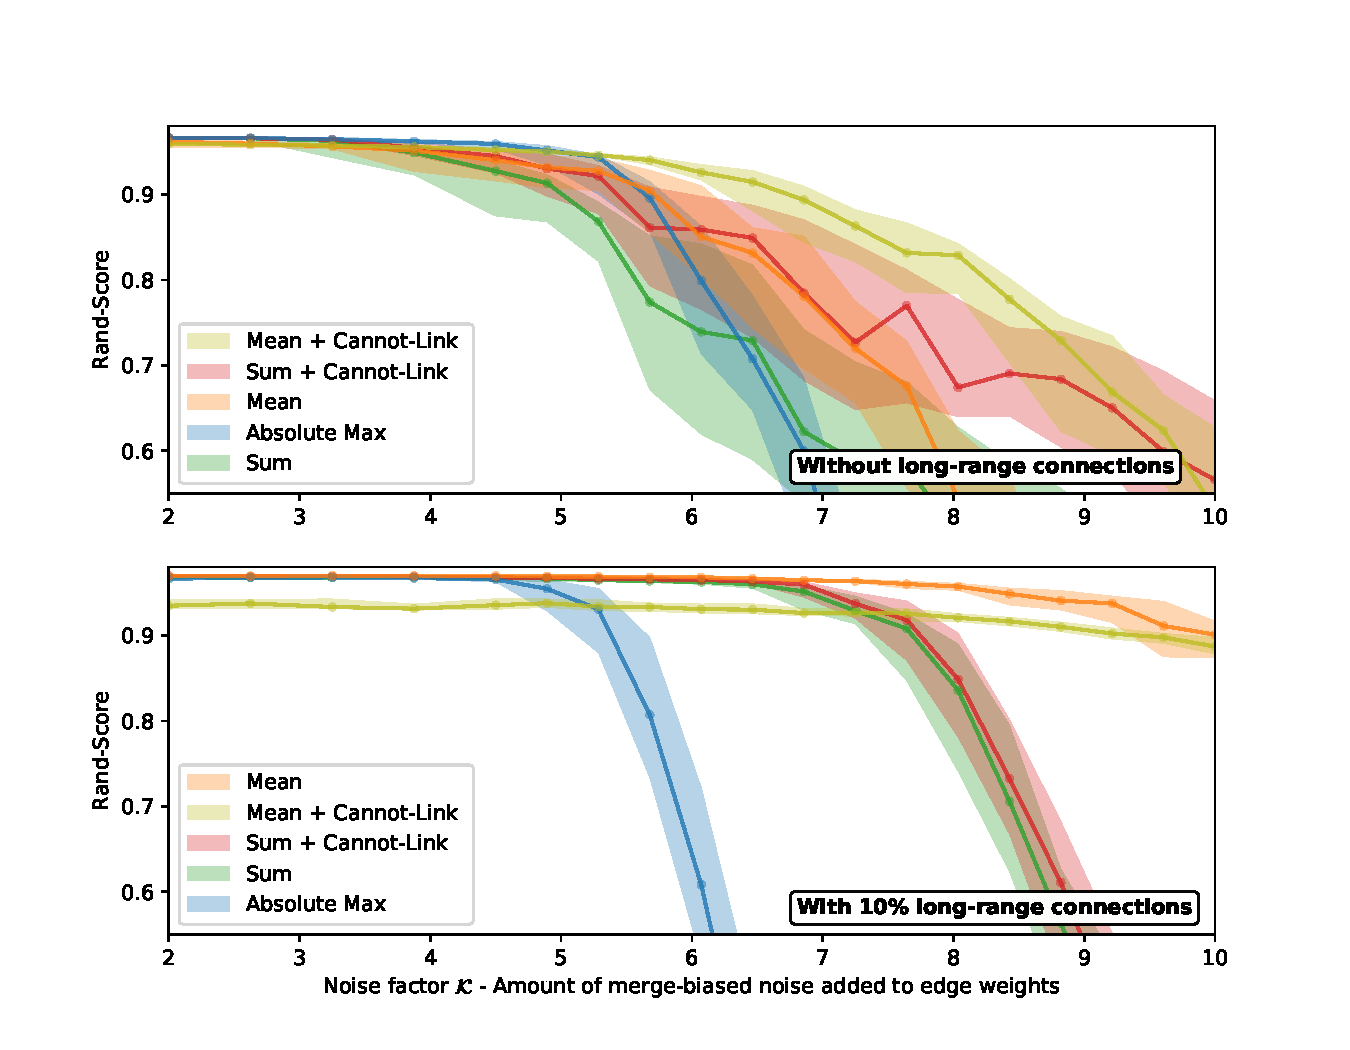
\includegraphics[width=0.98\textwidth,trim=0.35in 0.35in 0.35in 0.35in,clip]{./figs/merge_noise.pdf}

%         \captionof{subfigure}{Merge-biased opensimplex noise} \label{fig:thresh}
%     \end{minipage}\hfil
% \begin{minipage}[b]{0.48\textwidth}
%     % \end{subfigure}%
%     % \begin{subfigure}[t]{0.48 \textwidth}
%         \centering
%         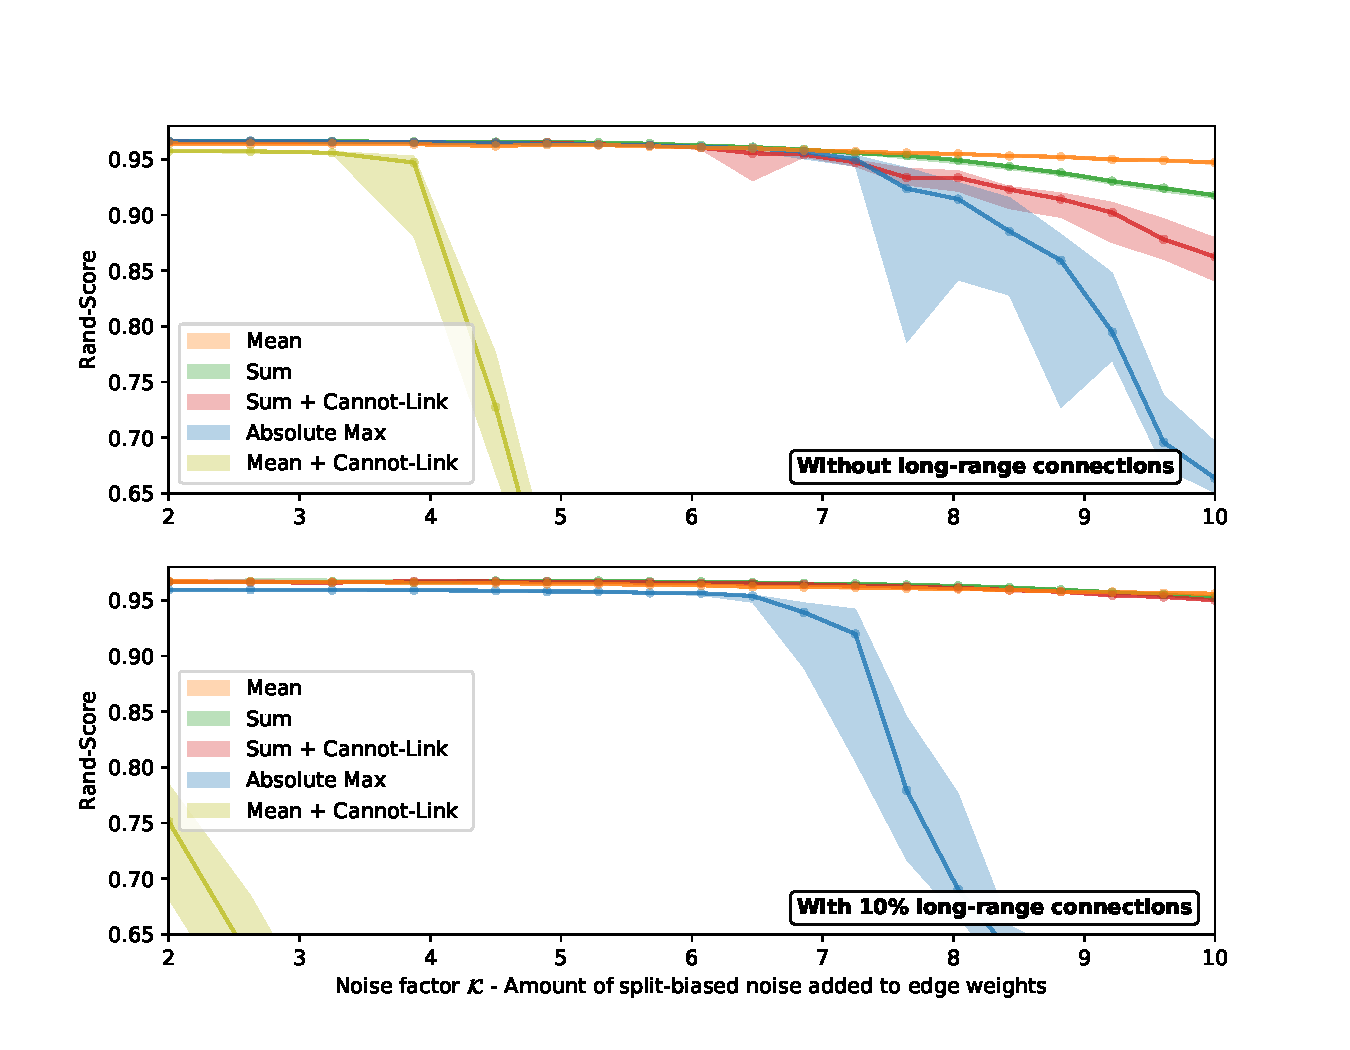
\includegraphics[width=0.98\textwidth,trim=0.29in 0.31in 0.31in 0.31in,clip]{./figs/split_noise.pdf}
%         \captionof{subfigure}{Split-biased opensimplex noise} \label{fig:ws}
%     % \end{subfigure}
% \captionof{figure}{Plot illustrating Adapted RAND scores achieved by UGACA and different update rules when noise is added to the edge weights... Solid lines represent median values, whereas values between the 25th and the 75th percentile are shown in shade areas.    \TODO{Label which uses only local-neighbors and which uses long-range connections}}\label{fig:noise_plots}
% % \end{figure}



\subsection{In-depth comparison of different linkage criteria for \algname{}}
Highlight difference of the sum in Fig. \ref{fig:intro_figure}.
% \begin{itemize}
%   % \item compare different choices of signed-cost-mappings (say which one worked best)
%   % \item present cremi crop-C table and rule out single and complete linkage
% \end{itemize}
Among the update rules listed in Table \ref{tab:linkage-criteria}, in the next sections we will only focus on \emph{sum}, \emph{arithmetic mean} and \emph{absolute maximum}, since they performed best in these experiments.


 In this section we evaluate the robustness of \algname{} with different linkage criteria by adding noise to the edge weights.
  %Before to present the results shown in Fig. \ref{fig:noise_plots}, we will first introduce the type of noise that was added to the edge weights.
% In the set of experiments presented in this article, edge weights are estimated \UPDATE{by using a CNN that predicts how likely two neighboring pixels are to be part of the same cluster}. 
Fig. \hyperref[fig:noisy_affs]{\ref*{fig:noisy_affs}a} shows an example of uncertain CNN predictions on a slice of the neuron segmentation dataset. We now present a way of modifying the CNN output to introduce additional artifacts like a missing or false boundary evidence. 

In the field of image processing there are several ways of adding noise to an image, among which the most common are Gaussian noise or Poisson shot noise. 
In these cases, the noise of one pixel does not correlate with its neighboring noise values. On the other hand, predictions of a CNN are known to be spatially correlated. 
Thus, we used Perlin noise\footnote{In our experiments, we used an open-source version of simplex noise \cite{perlin2001noise}, which is an improved open-source version of Perlin noise \cite{perlin1985image}}, one of the most common gradient noises used in procedural pattern generation. This type of noise $n(x)\in[0,1]$ generates spatial random patterns that are locally smooth but have large and diverse variations on bigger scales. We then combined it with the CNN predictions $p(x)$ in the two following ways: 
\begin{equation}\label{eq:noise_biased_predictions}
% \tilde{F}(x;\theta)=\begin{cases}
% F(x;\theta)+\mathcal{K}\cdot\max\left(N(x),0\right) & \text{if merge-biased}\\
% F(x;\theta)+\mathcal{K}\cdot\min\left(N(x),0\right) & \text{if split-biased}
% \end{cases}
\tilde{F}_{\pm}(x;\mathcal{K})=F(x)\pm\big|\mathcal{K}\cdot\max\left(\pm N(x),0\right)\big|,
\end{equation}
where  $N(x)=\mathrm{Logit}[n(x)]$; $F(x)=\mathrm{Logit}[p(x)]$ and $\mathcal{K}\in \mathbb{R}^+$ is a positive factor representing the amount of added noise. $\tilde{F}_{+}(x;\mathcal{K})$ represents then a merge-biased prediction, such that the probability for two pixels to be in the same cluster is increased only if $N(x)>0$ (see Fig. \hyperref[fig:noisy_affs]{\ref*{fig:noisy_affs}b}), whereas $\tilde{F}_{-}(x;\mathcal{K})$ is a split-biased prediction with decreased probabilities when $N(x)<0$ (Fig. \hyperref[fig:noisy_affs]{\ref*{fig:noisy_affs}c}). In the Supplementary material (Sec. \ref{sec:details_perlin}) we provide a more detailed description of the parameters used for the noise generation.
% \UPDATE{The plots in Fig. \ref{fig:noise_plots} represent the scores achieved by \algname{} with different update rules depending on the amount of noise $\mathcal{K}$ added to the edge weights and the probability $p_{\mathrm{long}}$ of long-range connections in the graph. Results clearly show that adding long-range edges is always beneficial for the final segmentation \TODO{Not True!}. \TODO{What about time?} The most robust version of update rule proved to be the \emph{mean}, that achieves similar scores even with significantly noisy edge weights. The \emph{absolute maximum} update rule proposed by \cite{wolf2018mutex} provides an efficient and fast option, but completely fails when too much noise is added. 
% The \emph{sum} update rule version was the slowest option tested, but it was not as robust as the \emph{mean} version, probably due to its tendency to grow one cluster at the time (see Sec. \ref{sec:exp_first_comparison}). \TODO{Comment about MC energy}
% On the other hand, \algname{} with \emph{mean} update rule and cannot-link constraints did not achieve high scores because of the strong over-segmentation error.}


\begin{figure}[b]
\centering
\begin{minipage}[T]{0.54\textwidth}
    \centering
    \footnotesize
        \begin{tabular}{l|l|cc}
           & \algname{}  &  \multicolumn{2}{c}{Use constraints:} \\
           & Linkage & \textsc{No} & \textsc{Yes} \\ \midrule
DWT \cite{bai2017deep} & - & 21.2 & - \\
SGN \cite{liu2017sgn} & - & 29.2 & - \\
Mask RCNN \cite{he2017mask} & - & 31.5 & - \\ \hline
 & Min &  0    & 0  \\
 & Sum \cite{keuper2015efficient,levinkov2017comparative} & 31.3  & 31.9  \\
\multirow{2}{*}{GMIS Pipeline \cite{liu2018affinity}} & Abs. Max. \cite{wolf2018mutex}  & 32.1 & 32.1 \\
 & Max &   24.3  &   32.5  \\
 & GMIS \cite{liu2018affinity} & 33.0 & -  \\
 & \textbf{Average}& \textbf{34.3}  & 33.9  \\
        \end{tabular}
    \captionof{table}{AP scores on the cityscapes validation set for the generalized algorithm and different types of linkage criteria.  }
    \label{tab:results_cityscapes_val}
\end{minipage}\hfill
\begin{minipage}[T]{0.43\textwidth}
    \centering
    \centering
\includegraphics[width=\textwidth]{./figs/cityscapes_compare_2.pdf} % left bottom right top
\end{minipage}
\end{figure}



% \begin{equation}
% \begin{gathered}
% \tilde{p}_{\pm}(x;\theta)=\sigma(\tilde{F}_{\pm}(x;\theta))\quad \text{where}\\
% % \tilde{F}(x;\theta)=\begin{cases}
% % F(x;\theta)+\mathcal{K}\cdot\max\left(N(x),0\right) & \text{if merge-biased}\\
% % F(x;\theta)+\mathcal{K}\cdot\min\left(N(x),0\right) & \text{if split-biased}
% % \end{cases}
% \tilde{F}_{\pm}(x;\theta)=F(x;\theta)\pm\left|\mathcal{K}\cdot\max\left(\pm N(x),0\right)\right|
% \end{gathered}
% \end{equation}
